The system implementation is divided into four main modules, Feature extraction, Pose estimation, Non-linear optimization and 3D visualization.

\begin{figure}[htb]
	\centering
	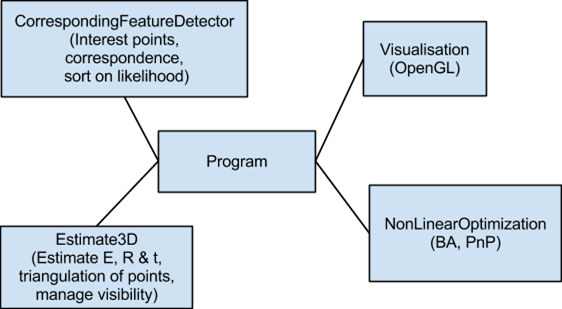
\includegraphics[width=110mm]{images/system_modules.png}
	\caption{\textit{Modules of the system}}
	\label{fig:block_overview2_fig}  %Skapar referens till figuren
\end{figure}

First feature extraction using SWIFT.... (preprocessing)

Then initial camera pose estimation + PnP and initial 3D-point triangulation of new unique 3D-points...

Then optimization over both camera poses and 3D-points (BA)...

When all camera poses and estimated 3D-points have been iteratively added and optimized the result is rendered using OpenGL.

\begin{figure}[htb]
	\centering
	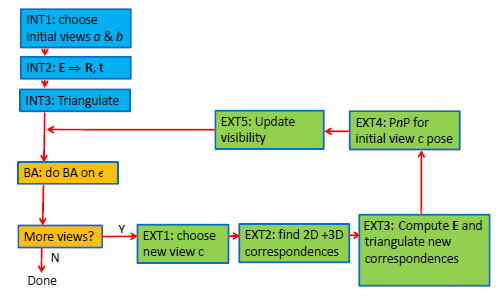
\includegraphics[width=120mm]{images/data_flow.png}
	\caption{\textit{Data flow between modules.}}
	\label{fig:block_overview_fig}  %Skapar referens till figuren
\end{figure}
